\setAuthor{Richard Luhtaru}
\setRound{lahtine}
\setYear{2024}
\setNumber{G 3}
\setDifficulty{3}
\setTopic{TODO}

\prob{Valguskaabel}
Silindriline sirge valguskaabel koosneb südamikust ja kattekihist ning selle ots on tasane ja kaabliga risti. Kui valgustada kaabli otsa välise valgusallikaga, siseneb osa välisest valgusest südamikku ja levib praktiliselt kadudeta pikki vahemaid. Seda, kui vastuvõtlik on valguskaabel välisele valgusele, iseloomustab numbriline apertuur (NA), mis on defineeritud kui $\text{NA} = \sin \theta_0$, kus $\theta_0$ on suurim välise valguskiire nurk (kaabli sümmeetriatelje suhtes), mis valguskaablisse sisenedes levib selle südamikus kadudeta. Leia valguskaabli numbriline apertuur NA, kui südamiku murdumisnäitaja on $n_1$, kattekihi murdumisnäitaja on $n_2$ ja kaabel asub välises keskkonnas murdumisnäitajaga $n_0$.
\begin{figure}[h]
    \centering
    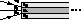
\includegraphics[width=.7\linewidth]{2024-lahg-03-yl.pdf}
\end{figure}




\hint

\solu
Defineerime nurgad $\alpha$ ja $\beta$ nagu joonisel. Valgus levib ilma kadudeta siis, kui $\beta$ on piisavalt suur ja kaabli südamikus toimub täielik sisepeegeldumine. Seega piirjuhul
\begin{equation*}
    n_1 \sin \beta = n_2.
\end{equation*}

\begin{figure}[h]
    \centering
    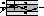
\includegraphics[width=.7\linewidth]{2024-lahg-03-sol.pdf}
\end{figure}

Murdumisseadusest saame samuti
\begin{equation*}
    n_0 \sin \theta_0 = n_1 \sin \alpha \implies n_0 \text{NA} = n_1 \sin \alpha \implies \text{NA} = \frac{n_1 \sin \alpha}{n_0}.
\end{equation*}

Kuna $\alpha$ ja $\beta$ on täisnurkse kolmnurga nurgad, siis $\beta = \ang{90} - \alpha$, seega $\sin \beta = \cos \alpha$. Seega
\begin{equation*}
    n_1 \cos\alpha = n_2 \implies \cos \alpha = \frac{n_2}{n_1} \implies \sin\alpha = \sqrt{1-\cos^2\alpha} = \sqrt{1-\left(\frac{n_2}{n_1}\right)^2}
\end{equation*}
ning
\begin{equation*}
    \text{NA} = \frac{n_1}{n_0}\sin\alpha = \frac{n_1}{n_0}\sqrt{1-\left(\frac{n_2}{n_1}\right)^2} = \frac{\sqrt{n_1^2-n_2^2}}{n_0}.
\end{equation*}
\probend